\documentclass{article}
\usepackage[a4paper, margin=1in]{geometry}
\usepackage[T1]{fontenc}
\usepackage[utf8]{inputenc}
\usepackage{amsmath, amssymb, graphicx, hyperref}
\graphicspath{{../figures/}}
\usepackage{bookmark}
\usepackage[framed,numbered]{matlab-prettifier}
\usepackage{xcolor}
\usepackage{listings}

\geometry{a4paper, margin=1in}

% MATLAB code style
\lstset{
  style      = Matlab-editor,
  basicstyle = \mlttfamily,
  breaklines = true
}

\title{\textbf{Practical - 6}}
\author{}
\date{October 17, 2026}

\pagenumbering{gobble}

\begin{document}
\maketitle

\noindent
\textbf{\large{Aim:}} To model exponential growth and decay problem.

\vspace{1em}
\noindent
\textbf{\large{Theory:}}

\vspace{0.5em}
\noindent
\textbf{Basic Model}
\[\frac{dy}{dt} = ky\]
where, 
\begin{flushleft}
    $y =$ quantity at time $t$ \\
    $t =$ time \\
    $k =$ growth/decay constant
\end{flushleft}

\vspace{1.5em}
\noindent
This model says that the rate of change of quantity is proportional to the quantity itself

\noindent
There arises two cases in this:

\noindent
\textit{\textbf{Case - I (Growth):}} If $k>0$, then the quantity increases.

\vspace{0.5em}
Example: \[\frac{dy}{dt} = 0.2y\]

\noindent
\textit{\textbf{Case - II (Decay):}} If $k<0$, then the quantity decreases.

\vspace{0.5em}
Example: \[\frac{dy}{dt} = -0.2y\]

\vspace{0.5em}
\noindent
So the model can describe both growth and decay.

\vspace{1.5em}
\noindent
\textbf{Mathematical Solution}

\noindent
Consider \[\frac{dy}{dt} = ky\]

\noindent
separating variables: \[\frac{dy}{y} = k\,dt\]

\noindent
integrating \[\ln{y} = kt + C\]

\noindent
Therefore, \[y = Ce^{kt}\]

\noindent
initial condition \[y(0) = y_o\]

\noindent
then \[y_oe^{kt}\]

\noindent
This is the formula for this practical

\noindent
\underline{Example:}
\[y(0) = 100, k = 0.2\]
thus the ODE is \[\frac{dy}{dt} = 0.2y\]
with \[y(0) = 100\]
the solution is \[y(t) = 100e^{0.2t}\]

\vspace{1em}
\noindent
\textbf{\large{MATLAB Code:}}
\begin{lstlisting}
clc; clear all; close all;

syms y(t)
eqn1 = diff(y) == 0.2*y;
init = y(0) == 100;
yGrowth = dsolve(eqn1, init);
disp(yGrowth)

eqn2 = diff(y, 1) == -0.2*y;
yDecay = dsolve(eqn2, init);
disp(yDecay)

fplot(yGrowth, [0, 10], 'LineWidth', 1.5)
hold on;
fplot(yDecay, [0, 10], 'LineWidth', 1.5)
grid on;
title('Exponential Growth and Decay')
xlabel('Time')
ylabel('Quantity')
legend('Growth', 'Decay')
\end{lstlisting}

\vspace{1em}
\noindent
\textbf{\large{Output:}}

\begin{flushleft}
$100\,{\mathrm{e}}^{t/5}$

$100\,{\mathrm{e}}^{-\frac{t}{5}}$
\end{flushleft}

\vspace{0.5em}

\begin{figure}[htbp]
    \centering
    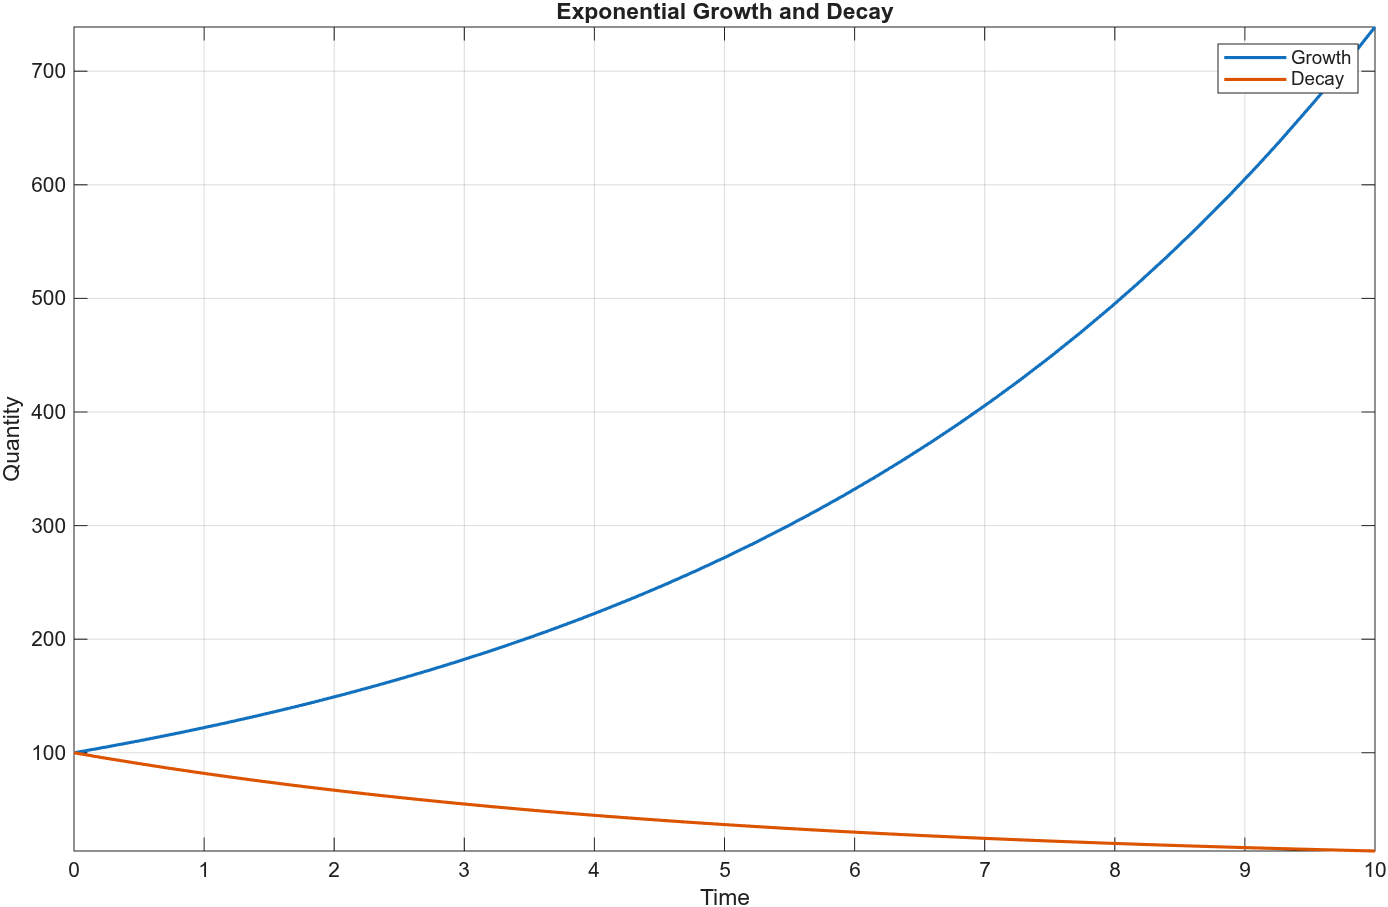
\includegraphics[width=0.7\textwidth]{Figure6.png}
\end{figure}

\end{document}
